%-------------------------------------------------------------------------------
% seq64_jack
%-------------------------------------------------------------------------------
%
% \file        seq64_jack.tex
% \library     Documents
% \author      Chris Ahlstrom
% \date        2016-01-28
% \update      2017-12-10
% \version     $Revision$
% \license     $XPC_GPL_LICENSE$
%
%     Provides the JACK page section of seq24-user-manual.tex.
%
%-------------------------------------------------------------------------------

\section{Sequencer64 JACK Support}
\label{sec:seq64_jack}

   This section describes some details concerning the JACK support of
   \textsl{Sequencer64}.
   As with \textsl{Seq24}, \textsl{Sequencer64} has JACK transport support.
   But, if one wants to use the older version of \textsl{Sequencer64} (versions
   0.9.x) with JACK MIDI, one needs to expose the ALSA ports to JACK using
   \texttt{a2jmidid --export-hw} and connect the resultant MIDI JACK ports
   oneself, using \textsl{QJackCtl}, for example.

   To enable the JACK transport support at run-time, the options
   \texttt{-j}/\texttt{--jack-transport}, \texttt{-J}/\texttt{--jack-master},
   and \texttt{-C}/\texttt{--jack-master-cond} are available.

   With version 0.90, \textsl{Sequencer64} can be built to support the legacy
   ALSA interface, the PortMIDI interface, or, best of all, the native JACK
   MIDI interface, loosely based on the RtMIDI project
   (see \cite{rtmidi}).  This mode also supports fallback-to-ALSA if the JACK
   server is not running.

   \begin{itemize}
      \item \textsl{Sequencer64}.
         \index{Sequencer64}.
         This application is built when the
         \texttt{--enable-alsamidi} option is specified at "configure" time.
         It is basically the 0.9.x version of \textsl{Sequencer64} application.
         However, this build is no longer the default.
      \item \textsl{seq64}.
         \index{seq64}.
         This application is built when the
         \texttt{--enable-rtmidi} option is specified at "configure" time.
         This build is now the default build.
      \item \textsl{seq64portmidi}.
         \index{seq64portmidi}.
         This application is built when the
         \texttt{--enable-portmidi} option is specified at "configure" time.
         This build is \textsl{deprecated}.  It works with Linux, but, for
         Windows support, we will instead add Windows API calls to the "rtmidi"
         build of the project.  We won't discuss this version at all.  We've
         tested it for playback, but nothing else.
   \end{itemize}

   The following sections discuss the JACK transport support and the native
   JACK MIDI support.

\subsection{Sequencer64 JACK Transport}
\label{subsec:seq64_jack_transport}

   This section is just underway.  Here are some of the topics to be discussed:

   \begin{enumerate}
      \item What JACK functions are supported for JACK Transport.
      \item Exposing the ALSA MIDI ports to JACK, when using the legacy
         ALSA version of \textsl{Sequencer64}.
      \item Fixes to JACK Master mode.
      \item Interactions with the Klick and Hydrogen applications.
      \item Patches from the new (!) version of Seq24, 0.9.3, to correct
         for MIDI Clock drift.
   \end{enumerate}

   In the meantime, the text files in the project's \texttt{contrib/notes}
   directory provide some useful setup notes.

   JACK transport support is \textsl{separate} from native JACK MIDI support.
   The JACK transport client is an invisible client with the
   name "seq64-transport", while the JACK MIDI client is visible in
   \textsl{QJackCtl}, and the ports created are part of the
   "seq64" client.

   The first thing to note about JACK transport with \textsl{Sequencer64} is
   that the progress bars will not move unless \textsl{Sequencer64} is
   connected to a JACK client, such as \textsl{Hydrogen} (in JACK MIDI mode)
   or \textsl{Yoshimi}.  Currently, \textsl{Sequencer64} will connect to a JACK
   client automatically only at startup, where it will connect to all JACK
   clients that it finds.  If it can't find a JACK client, then it will
   fail to register a JACK port, and cannot play.

   The second thing is that \textsl{Sequencer64} still has the issue where it
   must be JACK Master to follow transport.  More on this issue later.

\subsection{Sequencer64 Native JACK MIDI}
\label{subsec:seq64_jack_native_midi}

   This section discusses the new \textsl{seq64} application, which supports
   native JACK MIDI.  It is now the \textsl{official} version of
   \textsl{Sequencer64}, and new bugs will be fixed mainly in this version.

   The first thing to note about \textsl{seq64}
   is that it supports both ALSA and JACK
   MIDI.  If one runs it to support JACK, and JACK is not present, then
   \textsl{seq64}
   falls back to ALSA support.

   To run seq64 to support JACK, for now, one must add the
   \texttt{-t} or \texttt{--jack-midi}
   option.  Why \texttt{-t}?  We are running out of option letters.
   And eventually we will make the \texttt{-t} option the default.
   If \textsl{Sequencer64} (in its native JACK mode, using the
   \texttt{-t} or \texttt{--jack-midi} option)
   is run in JACK mode \textsl{without JACK running} on
   the system, it will take awhile to come up (in ALSA mode).  If run from the
   console, one will see:

\begin{verbatim}
	$ ./Seq64rtmidi/seq64 -t
	[Activating native JACK MIDI]
	[Reading rc configuration /home/ahlstrom/.config/sequencer64/sequencer64.rc]
	[Reading user configuration /home/ahlstrom/.config/sequencer64/sequencer64.usr]
	[Activating native JACK MIDI]
	Cannot connect to server socket err = No such file or directory
	Cannot connect to server request channel
	jack server is not running or cannot be started
     . . .
	[JACK server not running?]
	connect: JACK server not running?
	rtmidi_info: no compiled support for specified API     (???)
	[Initialized, running without JACK sync]
	9 rtmidi ports created:
	Input ports (3):
	  [0] 0:1 system:announce (system)
	  [1] 14:0 Midi Through:Midi Through Port-0
	  [2] 24:0 nanoKEY2:nanoKEY2 MIDI 1
	Output ports (6):
	  [0] 14:0 Midi Through:Midi Through Port-0 
	  [1] 24:0 nanoKEY2:nanoKEY2 MIDI 1 
	  [2] 128:0 TiMidity:TiMidity port 0 
	  [3] 128:1 TiMidity:TiMidity port 1 
	  [4] 128:2 TiMidity:TiMidity port 2 
	  [5] 128:3 TiMidity:TiMidity port 3 
\end{verbatim}

   To enable native JACK MIDI, use the
   \texttt{-t}/\texttt{--jack-midi} options.
   When enabled, the "transport" button in the main window will show the word
   "JACK" (no matter whether JACK transport is also enabled or not).
   Please note that, if you
   select the JACK-MIDI option and JACK is not available,
   \textsl{seq64} will start in
   ALSA mode and \textsl{it will save} that mode when exiting.

	\index{sticky options}
   The JACK (\texttt{-t}) and ALSA (\texttt{-A}) options are sticky options.
   That is, they are saved to the "rc" configuration file at exit,
   so one does not have to specify them in subsequent \textsl{seq64} sessions.

\subsubsection{Sequencer64 JACK MIDI Output}
\label{subsubsec:seq64_jack_midi_output}

   By default (or depending on the "rc" configuration file), the new
   \texttt{seq64} version of \textsl{Sequencer64} will
   \index{jack!auto-connect}
   \index{auto-connect}
   automatically connect the ports that it finds to \texttt{seq64},
   as shown in the following figure:

\begin{figure}[H]
   \centering 
   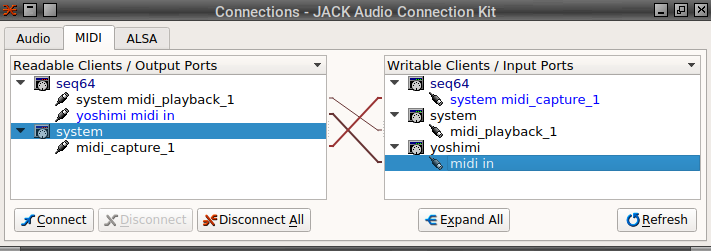
\includegraphics[scale=0.75]{jack/jack-nano-yosh-midi-auto-seq64.png}
   \caption{JACK MIDI Ports and Auto-Connect}
   \label{fig:seq64_jack_nano_yosh_midi_auto}
\end{figure}

   The \texttt{seq64:system midi\_playback\_1} output port shown
   in the left panel is created by \texttt{seq64}.  It connects it to the 
   \texttt{system:midi\_playback\_1} port in the right panel, which
   is actually the input for the \textsl{Korg nanoKEY2} controller.
   ALSA detects the real name of this USB MIDI device, but JACK does not.  
   Thus, the MIDI tab shows the "system" name of the USB MIDI port, while
   the ALSA tab does show the name.

\begin{figure}[H]
   \centering 
   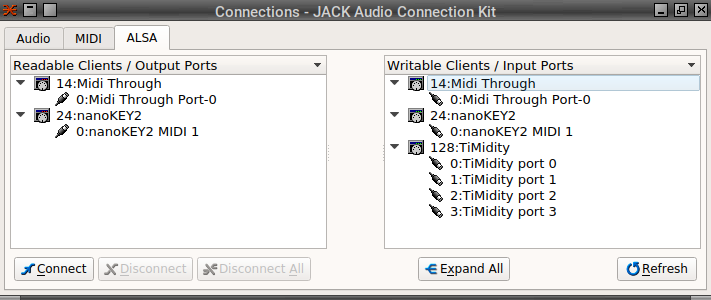
\includegraphics[scale=0.75]{jack/jack-nano-yosh-alsa-pre-seq64.png}
   \caption{ALSA MIDI Ports}
   \label{fig:seq64_jack_nano_yosh_alsa_pre}
\end{figure}

	Note that the input connection is not useful unless \texttt{seq64} could
   send setup information to the \textsl{nanoKEY2}.
   Korg provides a configuration application for \textsl{Windows}.
   For \textsl{Linux}, a Python application called \textsl{Nano-Basket}
	(\cite{nanobasket}) is available.

   More useful is the automatic connection between
   \texttt{seq64:yoshimi midi in} in the left (output) panel and
   \texttt{yoshimi:midi in} in the right (input) panel.  With it it,
   \textsl{Sequencer64} patterns with the proper output-buss setting can play
   to the \textsl{Yoshimi} software synthesizer.

	The output ports available are shown in \textsl{seq64}'s
	\textbf{File / Options / MIDI Clock} tab, shown here:

\begin{figure}[H]
   \centering 
   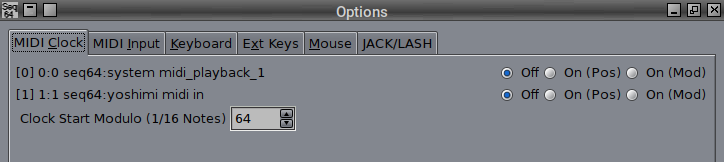
\includegraphics[scale=0.75]{jack/jack-nano-yosh-midi-clock-seq64.png}
   \caption{JACK MIDI Ports in Seq64}
   \label{fig:seq64_jack_nano_yosh_midi_clock}
\end{figure}

   Note that the index, client, and buss numbers are all the same.
   There's actually a bug here, since all \texttt{seq64} ports should have the
   same client number.  However, in JACK, clients and ports are referred to by
   name, not number, and so functionality is not affected.

   Entry 0 (\texttt{seq64:system midi\_playback\_1}) is,
   as already noted, not useful unless the \textsl{nanoKEY2} can
   accept input control.  Entry 1 allows \texttt{seq64} to send MIDI
   to \textsl{Yoshimi}.  A pattern must specify output buss 1 in order for the
   MIDI to reach \textsl{Yoshimi}.  Another option, normally for testing only,
   is to specify the "bus" option on the command line:

   \begin{verbatim}
      $ seq64 --jack-midi --bus 1
   \end{verbatim}

   With that option, all patterns send to buss 1.

\subsubsection{Sequencer64 JACK MIDI Input}
\label{subsubsec:seq64_jack_midi_input}

   One more connection to note is the input connection to \texttt{seq64}.
   Referring back to 
   \figureref{fig:seq64_jack_nano_yosh_midi_auto}
   we see that
   \texttt{system:midi\_capture\_1} in the left (output) panel is connected to
   \texttt{seq64:system midi\_capture\_1} in the right (input) panel.
   This allows the \textsl{nanoKEY2} MIDI output port to feed \texttt{seq64},
   which can then record the input notes, and also forward them to
   \textsl{Yoshimi} so that they can be heard.

   This input port is also shown in the \textbf{File / Options / MIDI Input}
   tab, shown here:

\begin{figure}[H]
   \centering 
   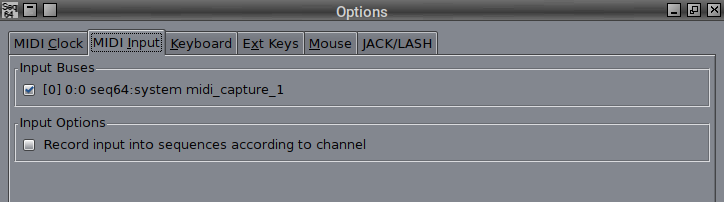
\includegraphics[scale=0.75]{jack/jack-nano-yosh-midi-input-seq64.png}
   \caption{JACK MIDI Input Ports}
   \label{fig:seq64_jack_nano_yosh_midi_input}
\end{figure}

   When the check-box for that buss is selected, the input can be captured by
   \texttt{seq64}.

\subsubsection{Sequencer64 JACK MIDI Virtual Ports}
\label{subsubsec:seq64_jack_midi_virtual_ports}

   \index{ports!manual}
   \index{ports!virtual}
   The manual-versus-normal port support for JACK MIDI is essentially the same
   as that for ALSA.  Currently, the same option name is used (we will provide
   a more generic option-name soon).
   The \texttt{-m}/\texttt{--manual-alsa-ports} option actually provides what
   are known as "virtual" ports.  These are ports that do not represent
   hardware, but are created by applications to allow them to connect to other
   applications or MIDI devices.

   The difference between manual/virtual ports and normal ports is that, while
   normal ports are automatically connected to the remote ports that exist in
   the system, the manual/virtual ports are just created, and one must
   manually connect them via, for example, the
   \textsl{QJackCtl} connections dialog.

   So, if one wants \textsl{seq64} to automatically connect to all existing
   JACK MIDI ports, \textsl{do not} use the
   \texttt{-m}/\texttt{--manual-alsa-ports} option... use the
   \texttt{-a}/\texttt{--auto-alsa-ports} option.  Both options apply to both
   ALSA and JACK, but we do not want to change the option-names at this time.

   If one wants the freedom to make the connections oneself, or with a session
   manager, then use the manual/virtual option.
   Here are the ports created in manual/virtual mode:

\begin{figure}[H]
   \centering 
   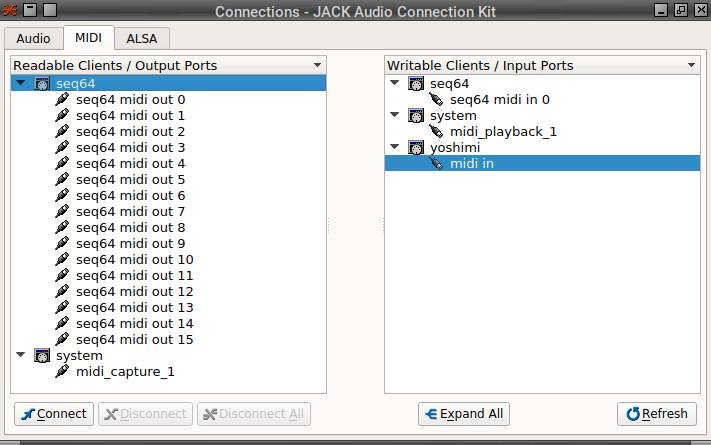
\includegraphics[scale=0.75]{jack/jack-nano-yosh-midi-manual-seq64.png}
   \caption{JACK MIDI Manual Ports}
   \label{fig:seq64_jack_nano_yosh_midi_manual}
\end{figure}

   One sees that \texttt{seq64} creates 16 output ports (busses), and one input
   port (buss).  One also sees that \texttt{seq64} \textsl{does not} connect
   the ports automatically.  The user or the session manager will have to make
   those connections.

   The \textbf{MIDI Clock} and \textbf{MIDI Input} tabs reflect in an obvious
   manner what is seen in \textsl{QJackCtl}, so we won't bother to show those
   tabs.

\subsubsection{Sequencer64 JACK MIDI and a2jmidid}
\label{subsubsec:seq64_jack_midi_a2jmidid}

   One more thing to show is that \texttt{seq64} can deal with the odd naming
   of JACK ports created by the \textsl{a2jmidid} application.

\begin{figure}[H]
   \centering 
   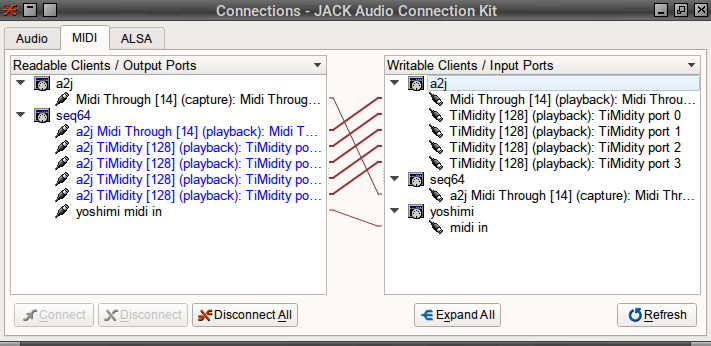
\includegraphics[scale=0.75]{jack/a2jmidid-jack-midi.png}
   \caption{JACK MIDI a2jmidid Ports}
   \label{fig:seq64_a2jmidid_jack_midi}
\end{figure}

   One can see in the right (input) panel that that the \texttt{a2j} client
   creates 5 entries, one for "Midi Through", and four for the
   \textsl{TiMidity} client.
   In the left (output) panel, one sees (in blue) the output
   ports that \texttt{seq64} creates to connect to the ports created by
   \textsl{a2jmidid}.

   Also note the true JACK output port,
   \texttt{seq64:yoshimi midi in} to connect to the input port
   \texttt{yoshimi:midi in}.

   Again, if these automatic connections get in the way, run \texttt{seq64} in
   manual/virtual mode.

   When recording, do not forget the step option.  If one paints notes with the
   mouse, the note is previewed, and the note position advances with each
   click.  If one paints notes via an external MIDI keyboard, the notes are
   painted and advanced, but they are not previewed.  To preview them, click
   the "pass MIDI in to output" button in the pattern editor window to activate
   so that they will be passed to your sound generator.
	Be careful of MIDI loops!

%-------------------------------------------------------------------------------
% vim: ts=3 sw=3 et ft=tex
%-------------------------------------------------------------------------------
